\documentclass[tikz, border=8pt]{standalone}
\usepackage{tikz}
\usepackage{xcolor}
\usepackage[T1]{fontenc}


\usetikzlibrary{
  arrows.meta,
  positioning,
  fit,
  backgrounds,
  shapes.geometric,
  shadows.blur
}

% ── Colour palette ────────────────────────────────────────────────────────────
\definecolor{col3d}{HTML}{1A5276}      % deep navy  — 3D branch
\definecolor{coltext}{HTML}{1E8449}    % forest green — text branch
\definecolor{colcca}{HTML}{6C3483}     % plum  — CCA / shared step
\definecolor{colout}{HTML}{784212}     % warm brown — output / eval
\definecolor{bglight}{HTML}{F4F6F7}    % near-white background panel
\definecolor{bggrey}{HTML}{EAF2FF}     % light blue tint for 3D panel
\definecolor{bggreen}{HTML}{EAFAF1}    % light green tint for text panel
\definecolor{arrowgrey}{HTML}{5D6D7E}  % neutral arrow colour

% ── Shared style definitions ──────────────────────────────────────────────────
\tikzset{
  %% Input nodes (raw data)
  inputnode/.style={
    rectangle, rounded corners=4pt,
    minimum width=3.2cm, minimum height=0.9cm,
    text centered, font=\small\bfseries,
    draw=#1!70!black, fill=#1!15,
    text=#1!60!black,
    blur shadow={shadow blur steps=5, shadow xshift=1pt, shadow yshift=-1pt,
                 shadow opacity=25}
  },
  %% Encoder boxes
  encbox/.style={
    rectangle, rounded corners=3pt,
    minimum width=3.2cm, minimum height=0.75cm,
    text centered, font=\small,
    draw=#1!60!black, fill=#1!20,
    text=#1!70!black
  },
  %% Dimension label (small badge on the right of encoder)
  dimlabel/.style={
    rectangle, rounded corners=2pt,
    minimum width=1.5cm, minimum height=0.5cm,
    text centered, font=\scriptsize\ttfamily,
    draw=#1!50!black, fill=#1!8,
    text=#1!80!black
  },
  %% Central processing step
  procbox/.style={
    rectangle, rounded corners=5pt,
    minimum width=4.2cm, minimum height=1.0cm,
    text centered, font=\small\bfseries,
    draw=#1!70!black, fill=#1!18,
    text=#1!60!black,
    blur shadow={shadow blur steps=5, shadow xshift=1pt, shadow yshift=-1pt,
                 shadow opacity=20}
  },
  %% Output / evaluation step
  outbox/.style={
    rectangle, rounded corners=5pt,
    minimum width=4.2cm, minimum height=0.9cm,
    text centered, font=\small\bfseries,
    draw=colout!70!black, fill=colout!12,
    text=colout!70!black
  },
  %% Section label (small italic text above group)
  seclabel/.style={
    font=\footnotesize\itshape,
    text=#1!65!black
  },
  %% Background panels
  bgpanel3d/.style={
    fill=bggrey, draw=col3d!25, rounded corners=6pt, line width=0.4pt
  },
  bgpaneltext/.style={
    fill=bggreen, draw=coltext!25, rounded corners=6pt, line width=0.4pt
  },
  %% Arrows
  mainarrow/.style={
    -{Latex[length=6pt, width=4pt]},
    line width=1.2pt, color=arrowgrey
  },
  mergarrow/.style={
    -{Latex[length=6pt, width=4pt]},
    line width=1.4pt, color=colcca!60!black
  }
}

\begin{document}
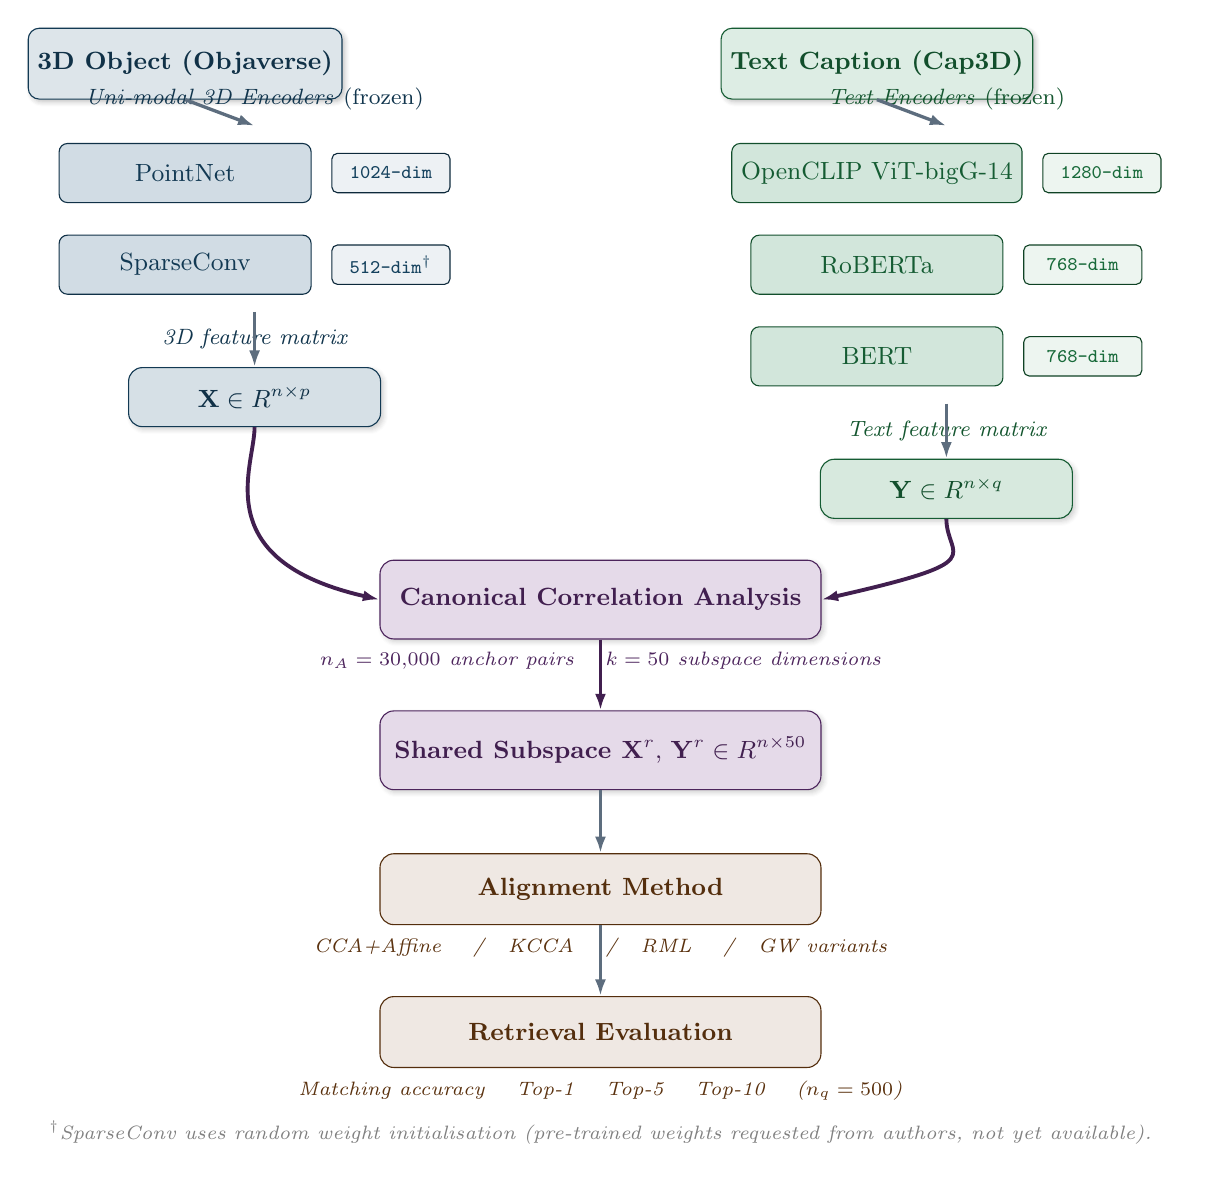
\begin{tikzpicture}[node distance=0.6cm and 1.6cm]

% ══════════════════════════════════════════════════════════════════════════════
% ROW 0  —  Input data
% ══════════════════════════════════════════════════════════════════════════════
\node[inputnode=col3d] (input3d)
  {3D Object (Objaverse)};

\node[inputnode=coltext, right=4.8cm of input3d] (inputtxt)
  {Text Caption (Cap3D)};

% ══════════════════════════════════════════════════════════════════════════════
% ROW 1  —  Encoders
% ══════════════════════════════════════════════════════════════════════════════

%% 3D encoders
\node[encbox=col3d, below=0.55cm of input3d] (pointnet)
  {PointNet};
\node[dimlabel=col3d, right=0.25cm of pointnet] (dpointnet)
  {1024-dim};

\node[encbox=col3d, below=0.40cm of pointnet] (sparseconv)
  {SparseConv};
\node[dimlabel=col3d, right=0.25cm of sparseconv] (dsparseconv)
  {512-dim$^{\dagger}$};

%% Text encoders
\node[encbox=coltext, below=0.55cm of inputtxt] (clip)
  {OpenCLIP ViT-bigG-14};
\node[dimlabel=coltext, right=0.25cm of clip] (dclip)
  {1280-dim};

\node[encbox=coltext, below=0.40cm of clip] (roberta)
  {RoBERTa};
\node[dimlabel=coltext, right=0.25cm of roberta] (droberta)
  {768-dim};

\node[encbox=coltext, below=0.40cm of roberta] (bert)
  {BERT};
\node[dimlabel=coltext, right=0.25cm of bert] (dbert)
  {768-dim};

% ══════════════════════════════════════════════════════════════════════════════
% Background panels around encoder groups
% ══════════════════════════════════════════════════════════════════════════════
\begin{scope}[on background layer]
  \node[bgpanel3d,
        fit=(pointnet)(sparseconv)(dpointnet)(dsparseconv),
        inner sep=6pt] (panel3d) {};

  \node[bgpaneltext,
        fit=(clip)(roberta)(bert)(dclip)(droberta)(dbert),
        inner sep=6pt] (paneltxt) {};
\end{scope}

% Section labels above panels
\node[seclabel=col3d, above=2pt of panel3d]
  {Uni-modal 3D Encoders \emph{(frozen)}};
\node[seclabel=coltext, above=2pt of paneltxt]
  {Text Encoders \emph{(frozen)}};

% ══════════════════════════════════════════════════════════════════════════════
% ROW 2  —  Feature matrices (intermediate)
% ══════════════════════════════════════════════════════════════════════════════
\node[procbox=col3d,
      below=0.7cm of panel3d,
      minimum width=3.2cm, minimum height=0.75cm,
      font=\small] (feat3d)
  {$\mathbf{X} \in \mathbb{R}^{n \times p}$};

\node[procbox=coltext,
      below=0.7cm of paneltxt,
      minimum width=3.2cm, minimum height=0.75cm,
      font=\small] (feattxt)
  {$\mathbf{Y} \in \mathbb{R}^{n \times q}$};

\node[seclabel=col3d, above=3pt of feat3d]   {3D feature matrix};
\node[seclabel=coltext, above=3pt of feattxt] {Text feature matrix};

% ══════════════════════════════════════════════════════════════════════════════
% ROW 3  —  CCA (central)
% ══════════════════════════════════════════════════════════════════════════════
% Horizontal centre between the two feature nodes
\coordinate (midpoint) at ($(feat3d.south east)!0.5!(feattxt.south west)$);

\node[procbox=colcca,
      below=1.1cm of midpoint,
      minimum width=5.6cm] (cca)
  {Canonical Correlation Analysis};

% Anchor note below CCA box
\node[font=\scriptsize\itshape, text=colcca!70!black,
      below=1pt of cca]
  {$n_A = 30{,}000$ anchor pairs \quad $k = 50$ subspace dimensions};

% ══════════════════════════════════════════════════════════════════════════════
% ROW 4  —  Shared subspace
% ══════════════════════════════════════════════════════════════════════════════
\node[procbox=colcca,
      below=0.9cm of cca,
      minimum width=5.6cm] (subspace)
  {Shared Subspace
   $\mathbf{X}^r,\, \mathbf{Y}^r \in \mathbb{R}^{n \times 50}$};

% ══════════════════════════════════════════════════════════════════════════════
% ROW 5  —  Alignment / Evaluation
% ══════════════════════════════════════════════════════════════════════════════
\node[outbox,
      below=0.8cm of subspace,
      minimum width=5.6cm] (align)
  {Alignment Method};

\node[font=\scriptsize\itshape, text=colout!75!black,
      below=1pt of align]
  {CCA+Affine \quad/\quad KCCA \quad/\quad RML \quad/\quad GW variants};

\node[outbox,
      below=0.9cm of align,
      minimum width=5.6cm] (eval)
  {Retrieval Evaluation};

\node[font=\scriptsize\itshape, text=colout!75!black,
      below=1pt of eval]
  {Matching accuracy \quad Top-1 \quad Top-5 \quad Top-10 \quad ($n_q = 500$)};

% ══════════════════════════════════════════════════════════════════════════════
% ARROWS
% ══════════════════════════════════════════════════════════════════════════════

%% Input → encoder group panels
\draw[mainarrow] (input3d.south)  -- (panel3d.north);
\draw[mainarrow] (inputtxt.south) -- (paneltxt.north);

%% Encoder panels → feature matrices
\draw[mainarrow] (panel3d.south)  -- (feat3d.north);
\draw[mainarrow] (paneltxt.south) -- (feattxt.north);

%% Feature matrices → CCA (converging arrows)
\draw[mergarrow] (feat3d.south)
    .. controls +(0,-0.5) and +(-2.2,0.5) .. (cca.west);
\draw[mergarrow] (feattxt.south)
    .. controls +(0,-0.5) and +(2.2,0.5) .. (cca.east);

%% CCA → shared subspace → alignment → evaluation
\draw[mergarrow] (cca.south)      -- (subspace.north);
\draw[mainarrow] (subspace.south) -- (align.north);
\draw[mainarrow] (align.south)    -- (eval.north);

% ══════════════════════════════════════════════════════════════════════════════
% FOOTNOTE
% ══════════════════════════════════════════════════════════════════════════════
\node[font=\scriptsize\itshape, text=gray,
      below=0.55cm of eval, xshift=0cm]
  {$^{\dagger}$SparseConv uses random weight initialisation
   (pre-trained weights requested from authors, not yet available).};

\end{tikzpicture}
\end{document}